\documentclass[english,twocolumn,DIV21,a4,10pt]{scrartcl}
\usepackage{babel}
\usepackage{amsmath}
\usepackage{graphicx}
\usepackage{units}
\usepackage{nomencl} 
\usepackage{color}

\newcommand{\dr}{\Delta_\textrm{R}}
%\newcommand{\eqref}{1}{(\ref{#1})}
\newcommand{\dc}{{}^\circ\textrm{C}}


\makenomenclature
\begin{document}
\title{Kommentare zum Praktikumsversuch: Heterogenes chemisches Gleichgewicht}
\author{Martin Kielhorn}
\maketitle
\section{Ziel des Versuches:}
Es ist das Massenwirkungsgesetz auf das Zersetzungsgleichgewicht eines
Nickel-Hexamin-Komplexes anzuwenden. Aus der Temperaturabhängigkeit
der Gleichgewichtskonstanten sind die Standardreaktionsenergie, die
Standardreaktionsenthalpie sowie die Standardreaktionsentropie zu
ermitteln.
\section{Begriffe}
\printnomenclature
\subsection{Thermodynamisches Potential}
\subsection{Thermodynamisches Gleichgewicht}
\begin{itemize}
\item konstante Temperatur, konstanter Druck: $\dr G = 0$
\item konstantes Volumen $\dr F = 0$
\end{itemize}
\section{Theoretische Grundlagen}
Bei einigen Ammoniak-Additionsverbindungen stellt sich umkehrbar und
relativ schnell ein Zersetzungsgleichgewicht ein. Beispielsweise kann
festes Ni-Hexaminchlorid mit festem Diaminchlorid und Ammoniak in
der Gasphase im Gleichgewicht stehen:

\begin{align}
  \label{eqn:hex}
  \underbrace{[Ni(NH_3)_6]Cl_2}_s \rightarrow 
  \underbrace{[Ni(NH_3)_2]Cl_2}_s + \underbrace{4 NH_3}_g
\end{align}

Da feste (s) und gasförmige (g) Phasen beteiligt sind, spricht man von
einem ``heterogenen Gleichgewicht''.  Das Massenwirkungsgesetz für
Gl.\eqref{eqn:hex} lautet:
\begin{align}
  K(T) = \frac{a_\textrm{Diamin} \cdot a^4_{NH_3}}{a_\textrm{Hexamin}}
\end{align}
wobei $a$ die \nomenclature{Aktivit\"at}{bla} Aktivit\"aten der
jeweiligen Stoffe und $K(T)$ die temperaturabhängige
Gleichgewichtskonstante sind. Solange die beteiligten Feststoffe in
reinen Phasen nebeneinander vorliegen (und nicht etwa als feste
L\"osung der einen Substanz in der anderen, wobei der Molenbruch jeder
Substanz kleiner als 1 w\"are), ist die Molenbruchaktivit\"at gleich
1.  Wird als Standardzustand des gasförmigen $NH_3$ das ideale Gas
unter einem Druck von $p = \unit[10^5]{Pa} = \unit[1]{Bar}$ gewählt,
ist die Aktivit\"at
\begin{align}
  a_{NH_3}=\frac{p_{NH_3}}{p^\theta},
\end{align}
so dass das Massenwirkungsgesetz die einfache Form
\begin{align}
  K(T)=\left(\frac{p_{NH_3}}{p^\theta}\right)^4
\end{align}
annimmt. Die Temperaturabhängigkeit der Gleichgewichtskonstanten
ergibt sich direkt aus der Messung des $NH_3-$Gleichgewichtsdruckes
als Funktion der Temperatur.

\begin{figure}
  \centering
  % \input{kapillare.eps_tex}
  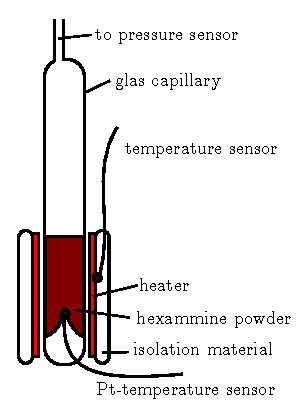
\includegraphics{kapillare.eps}
  \caption{Sketch of the setup. The hexamine powder is hermetically
    sealed and can be heated to constant temperature using an embedded
    semiconductor temperature sensor. There is also a more precise
    resistive temperature sensor close to the center of the powder.}
   \label{fig:kapillare}
 \end{figure}


Der Versuch wird bei konstantem Volumen durchgeführt. Für die
Gleichgewichtskonstante $K$ gilt dann folgende Beziehung (Lehrbücher
der Physikal. Chemie):
\begin{align}
  \label{eqn:frei}
  \dr F^\theta = -RT\ln K.
\end{align}
Unter Verwendung der Gibbs-Helmholtz-Gleichung
\begin{align}
  \label{eqn:frei2}
  \dr F^\theta = \dr U^\theta - T \cdot \dr S^\theta
\end{align}
ergibt sich
\begin{align}
  \ln K = -\frac{\dr U^\theta}{R}\frac{1}{T} + \frac{\dr S^\theta}{R}.
\end{align}
Unter der (im benutzten engen Temperaturintervall in guter Näherung
erfüllten) Voraussetzung, dass RU und R S temperaturunabhängig sind,
hängt $\ln K$ also linear von $1/T$ ab. Wenn $K$ als Funktion der
Temperatur gemessen und $\ln K$ als Funktion $1/T$ graphisch
dargestellt wird, kann man aus dem Anstieg bzw. Ordinatenabschnitt der
sich ergebenden Geraden $\dr U^\theta$ und $\dr S^\theta$
erhalten. Dazu ist es zweckmäßig, einige Umformungen
durchzuführen. (Im folgenden werden die Indizes $NH_3$ weggelassen.)

Wir ersetzen $\ln K$ mit $\ln K=4\ln(p/p^\theta)$ und Normaldruck
$p^\theta = \unit[10^5]{Pa}$ und erhalten eine lineare Gleichung in $y
= \ln(p/p^\theta)$ und $x=1/T$:
\begin{align}
  \label{eqn:fit}
  \underbrace{\ln \left(\frac{p(T)}{p^\theta}\right)}_y &= 
  \underbrace{\frac{\dr S^\theta}{4R}}_A \underbrace{-\frac{\dr U^\theta}{4R}}_B
  \frac{1}{T} \\
  y(x) &= A+B x
\end{align}
Aus den dimensionslosen Fit-Parameter $A$ und dem Parameter $B$ (in
${}^\circ\textrm{K}$) können die Standardreaktionsenthalpie $\dr
S^\theta$ und die \"Anderung der inneren Energie bei
Standardbedingungen $\dr U^\theta$ berechnet werden.

Der lineare Fit ermoeglicht die Bestimmung der
Gleichgewichtskonstanten $K(T)$ f\"ur beliebige Temperaturen und auch
die freie Standardreaktionsenergie $\dr F^\theta$.

\paragraph{Note:}
A constant pressure in reaction \ref{eqn:hex} corresponds to the
equilibrium in the free enthalpy $\dr G=0$. In this case equations
\eqref{eqn:frei} and \eqref{eqn:frei2} are replaced by
\begin{align}
  \dr G^\theta &= -RT \ln K \\
  \ln K &= - \frac{\dr H^\theta}{R} \frac{1}{T} + \frac{\dr S^\theta}{R}
\end{align}
The enthalpy $\dr H^\theta=\dr U^\theta + p \dr V^\theta$ contains an
additional term that corresponds to the work that is necessary to
increase the volume of the gas. The ideal gas equations are a good
approximation for $NH_3$ and we can determine the work. According to
\eqref{eqn:hex}, \unit[1]{mol} of hexamin reacts to \unit[4]{mol} of
$NH_3$ gas.
\begin{align}
  \dr V&= 4V_{NH_3}=4RT/p.
\end{align}
\section{Tasks}
\begin{enumerate}
\item Measure the disassociation pressure of hexamine $p$ for eight
  temperatures $T\in (90\ldots150^\circ\textrm{C})$.
\item Display the measured values and a linear fit according to
  equation \eqref{eqn:fit}.
\item Determine molar reaction enthalpy $\dr U^\theta$ and entropy
  $\dr S^\theta$ using the fit parameters $A$ and $B$.
\item Calculate the molar free reaction energy $\dr F^\theta(T)$, the
  equilibrium constant $K(T)$ and the molar reaction enthalpy $\dr
  H^\theta(T)$ for $T\in\{25\dc,75\dc,125\dc,175\dc\}$.
\end{enumerate}

\section{Measurement}

  \begin{table}[htbp]
    \centering
    \begin{tabular}{rr}
 T/${}^\circ\textrm{C}$ & p/mbar\\
  21.0 &  20 \\
  59.3 &  40 \\
  88.2 & 120 \\
 103.0 & 140 \\
 109.1 & 158 \\
 118.4 & 218 \\
 126.6 & 275 \\
 129.3 & 302 \\
 130.3 & 318 \\
 132.7 & 343 \\
 138.1 & 408 \\
 143.2 & 495 \\
 142.1 & 515 \\
 115.0 & 335 \\
  98.3 & 215 \\
  87.0 & 142 \\
  80.4 & 110 \\
  78.0 & 100 \\
  74.3 &  90 \\
  70.4 &  80 \\
  65.8 &  70 \\
  64.8 &  63 \\
    \end{tabular}
    \caption{Pressures for various temperatures.}
    \label{tab:meas}
  \end{table}
  The powder was heated to \unit[140]{${}^\circ\textrm{C}$}.  The
  pressure was measured at stable temperature points (the resistive
  temperature measurement shouldn't change anymore). The data is
  displayed in table \ref{tab:meas}.

  It was not possible to heat the powder to more than
  \unit[145]{${}^\circ\textrm{C}$}. Subsequently the temperature was
  lowered again and occasionally stabilized to measure more pressures.

  \begin{figure}[htbp]
    \centering
    \includegraphics{p1.eps}
    \caption{Pressures for various temperatures, connected in the sequence of measurement.}
    \label{fig:meas}
  \end{figure}

\section{Evaluation}
Figure \ref{fig:eval} displays the data in the linearization scheme
according to equation \eqref{eqn:fit}. The linear fit delivers the
parameters $A=2.47\pm0.4$ and
$B=\unit[(-3302\pm160)]{{}^\circ\textrm{K}}$.
  \begin{figure}[htbp]
    \centering
    \includegraphics{p2.eps}
    \caption{Measured data according to the linarization scheme.}
    \label{fig:eval}
  \end{figure}

%a               = 2.47621          +/- 0.4353       (17.58%)
%b               = -3302.25         +/- 160.1        (4.847%)

  With $R=\unit[8.314]{\textrm{J}/(\textrm{mol K})}$ we obtain
  $\Delta_R S=\unit[(82\pm14)]{\textrm{J}/(\textrm{mol K})}$ and
  $\Delta_R U = \unit[(10\pm5)]{\textrm{kJ}/(\textrm{mol K})}$.

% (* 4 8.314 2.47) (* .1758 4 8.314 2.47)
% (* 4 8.314 3302.25) (* .04847 4 8.314 3302.25)
\section{Discussion}
The diagram in figure \ref{fig:meas} indicates, that there occured a
strong hysteresis during the measurement. This is due to a major flaw
in the setup. The apparatus is only heated in a small area surrounding
the powder. The created $NH_3$ gas immediatly leaves the vincinity of
the heater and cools close to room temperature in the glass capillary
and the pressure sensor.

This slowly increases the temperature of the apparatus. Therefor the
measured gas pressures are higher when the temperature is lowered
again.

Trying to correcting for the effects of the cooling gas would involve
measuring the gas temperature and estimating the temperature gradients
and volumes within the apparatus. As this strongly depends on the
geometry of the apparatus, it seems to be not worth the effort.
Instead the setup should be improved, so that the whole measurement
volume has the same temperature.

\end{document}
